

\chapter{ETCS data packets}
\label{cha:packets}

In the following, we give a top-down presentation of the OpenETCS
Decoder software.
We discuss the highest, i.e.\ the data packet level, in this chapter;
Chapter~\ref{cha:bitstream} elaborates on some intermediate, and
Chapter~\ref{cha:low-level bitstream} on the lowest level.

On the data packet level, a total of 47 different packets
are defined as \isoc~\inl{struct}.
We exemplify our discussion on the alphabetically first packet,
\inl{AdhesionFactor} (Section~\ref{sec:adhesionfactor}), and give some
comments on considerations with respect to other packets
(Section~\ref{sec:other-packets}).

In order to cope with the similarity of specification, implementation,
and verification tasks for all packets, we have chosen to automatically 
generate formal specifications and implementations for encoding
and decoding data packets from chapter 7 of the
ETCS Subset 026 system requirements description.

\section{Overview and classification of data packets}
\label{sec:data-packets}

Tables~\ref{tbl:packets-packetnumbers-tracktotrain-part1},
\ref{tbl:packets-packetnumbers-tracktotrain-part2},
\ref{tbl:packets-packetnumbers-traintotrack}, and
\ref{tbl:packets-packetnumbers-bothways}
list the packets from ETCS requirements specification ``Subset~026''.
%
While many packets only contain a fixed number of elements, there
are also a few that contain a \emph{dynamic} number of elements
(indicated by the presence of a field \inl{N_ITER}) and \emph{optional} values.
We use the following terminology:

\begin{itemize}
\item
A packet that does not contain an element \inl{N_ITER} is
referred to as \emph{static packet}.

\item 
All other packets are referred to as \emph{dynamic packets}.
\end{itemize}

There are 29 static packets and 19 dynamic packets.
Seven of the 29 static packets contain optional values.

\begin{table}[hbt]
\begin{center}
\begin{tabular}{|m{8ex}|m{8cm}|c|c|c|}
\hline
PacketID & Packet name & \inl{N_ITER} & Optional\\
\hline
\hline
3 & National Values & + & +\\
\hline
5 & Linking & + & +\\
\hline
12 & Level 1 Movement Authority & + & -\\
\hline
15 & Level 2/3 Movement Authority & + & -\\
\hline
16 & Repositioning Information & - & -\\
\hline
21 & Gradient Profile & + & -\\
\hline
27 & International Static Speed Profile & + & -\\
\hline
39 & Track Condition Change of traction power & - & -\\
\hline
41 & Level Transition Order & + & +\\
\hline
42 & Session Management & - & +\\
\hline
44 & Data used by applications outside the ERTMS/ETCS system & - & -\\
\hline
45 & Radio Network registration & - & -\\
\hline
46 & Conditional Level Transition Order & + & +\\
\hline
49 & List of balises for SH Area & + & +\\
\hline
51 & Axle load Speed Profile & + & -\\
\hline
57 & Movement Authority Request Parameters & - & -\\
\hline
58 & Position Report Parameters & + & -\\
\hline
63 & List of Balises in SR Authority & + & +\\
\hline
65 & Temporary Speed Restriction & - & -\\
\hline
66 & Temporary Speed Restriction Revocation & - & -\\
\hline
67 & Track Condition Big Metal Masses & + & -\\
\hline
68 & Track Condition & + & +\\
\hline
70 & Route Suitability Data & + & +\\
\hline
71 & Adhesion Factor & - & -\\
\hline
72 & Packet for sending plain text messages & - & +\\
\hline
76 & Packet for sending fixed text messages & - & +\\
\hline
79 & Geographical Position Information & + & +\\
\hline
80 & Mode profile & + & -\\
\hline
90 & Track Ahead Free up to level 2/3 transition location & - & + \\
\hline
131 & RBC transition order & - & -\\
\hline
\end{tabular}
\end{center}
\caption{\label{tbl:packets-packetnumbers-tracktotrain-part1} TrackToTrain packets part 1}
\end{table}


\FloatBarrier  % forces the output of listings/tables

\begin{table}[hbt]
\begin{center}
\begin{tabular}{|m{8ex}|m{7cm}|c|c|}
\hline
PacketID & Packet name & \inl{N_ITER} & Optional\\
\hline
\hline
132 & Danger for Shunting information & - & -\\
\hline
133 & Radio in-fill area information & - & -\\
\hline
134 & EOLM Packet & - & -\\
\hline
136 & Infill location reference & - & +\\
\hline
137 & Stop if in Staff Responsible & - & -\\
\hline
138 & Reversing area information & - & -\\
\hline
139 & Reversing supervision information & - & -\\
\hline
140 & Train running number from RBC & - & -\\
\hline
141 & Default Gradient for Temporary Speed Restriction & - & -\\
\hline
254 & Default balise, loop or RIU information & - & -\\
\hline
\end{tabular}
\end{center}
\caption{\label{tbl:packets-packetnumbers-tracktotrain-part2} TrackToTrain packets part 2}
\end{table}

\FloatBarrier  % forces the output of listings/tables

\begin{table}[hbt]
\begin{center}
    \begin{tabular}{|m{8ex}|m{8cm}|c|c|}
\hline
               PacketID & Packet name & \inl{N_ITER} & Optional \\
\hline
\hline
0 & Position Report & - & +\\
\hline
1 & Position Report based on two balise groups & - & +\\
\hline
3 & Onboard telephone numbers & + & -\\
\hline
4 & Error Reporting & - & -\\
\hline
9 & Level 2/3 transition information & - & -\\
\hline
11 & Validated train data & + & -\\
\hline
44 & Data used by applications outside the ERTMS/ETCS system & - & -\\
\hline
\end{tabular}
\end{center}
\caption{\label{tbl:packets-packetnumbers-traintotrack} TrainToTrack packets}
\end{table}

%\FloatBarrier  % forces the output of listings/tables

\begin{table}[hbt]
\begin{center}
    \begin{tabular}{|m{8ex}|m{8cm}|c|c|}
\hline
               PacketID & Packet name & \inl{N_ITER} & Optional \\
\hline
\hline
255 & End of information & - & -\\
\hline
\end{tabular}
\end{center}
\caption{\label{tbl:packets-packetnumbers-bothways} Both-Ways packets}
\end{table}

\clearpage


\section{Formal specification of \inl{AdhesionFactor}}
\label{sec:adhesionfactor}

In this section we describe in detail the formal specification
of encoding and decoding operations of the packet \adhesion,
which is a typical static packet.

\subsection{\inl{AdhesionFactor} in ETCS}
\label{sec:adhesionfactor-etcs}

ETCS Subset~026 defines the package \emph{adhesion factor} (packet 71) as shown in 
Table~\ref{tbl:adhesion-factor}.

\begin{table}[hbt]
\begin{center}
\begin{tabular}{|l|r|}
\hline
\textbf{variable name} & \textbf{number of bits}\\
\hline
\inl{NID_PACKET} & 8 \\
\hline
\inl{Q_DIR} & 2 \\
\hline
\inl{L_PACKET} & 13 \\
\hline
\inl{Q_SCALE} & 2 \\
\hline
\inl{D_ADHESION} & 15 \\
\hline
\inl{L_ADHESION} & 15 \\
\hline
\inl{M_ADHESION} & 1 \\
\hline
\end{tabular}
\end{center}
\caption{\label{tbl:adhesion-factor} Packet \adhesion as defined by ETCS}
\end{table}


\subsection{The type \inl{AdhesionFactor}}
\label{sec:adhesionfactor-type}

Listing~\ref{lst:adhesionfactor-type} shows the definition of type
\inl{AdhesionFactor} as it is generated from the ETCS specification shown in Section~\ref{sec:adhesionfactor-etcs}.

\begin{listing}[hbt]
\begin{minipage}{0.99\textwidth}
\begin{lstlisting}[style=acsl-block]
struct AdhesionFactor
{
    PacketHeader header;

    // TransmissionMedia=Any
    // This packet is used when the trackside requests a change of
    // the adhesion factor to be used in the brake model.
    // Packet Number = 71

    uint64_t  Q_DIR;            // # 2
    uint64_t  L_PACKET;         // # 13
    uint64_t  Q_SCALE;          // # 2
    uint64_t  D_ADHESION;       // # 15
    uint64_t  L_ADHESION;       // # 15
    uint64_t  M_ADHESION;       // # 1
};

typedef struct AdhesionFactor AdhesionFactor;
\end{lstlisting}
\end{minipage}
\caption{\label{lst:adhesionfactor-type}Definition of the type \inl{AdhesionFactor}}
\end{listing}

\clearpage

Figure~\ref{fig:adhesionfactor-bitstream} outlines the mapping between 
a bit stream and the elements of \adhesion.

\begin{figure}
\begin{center}
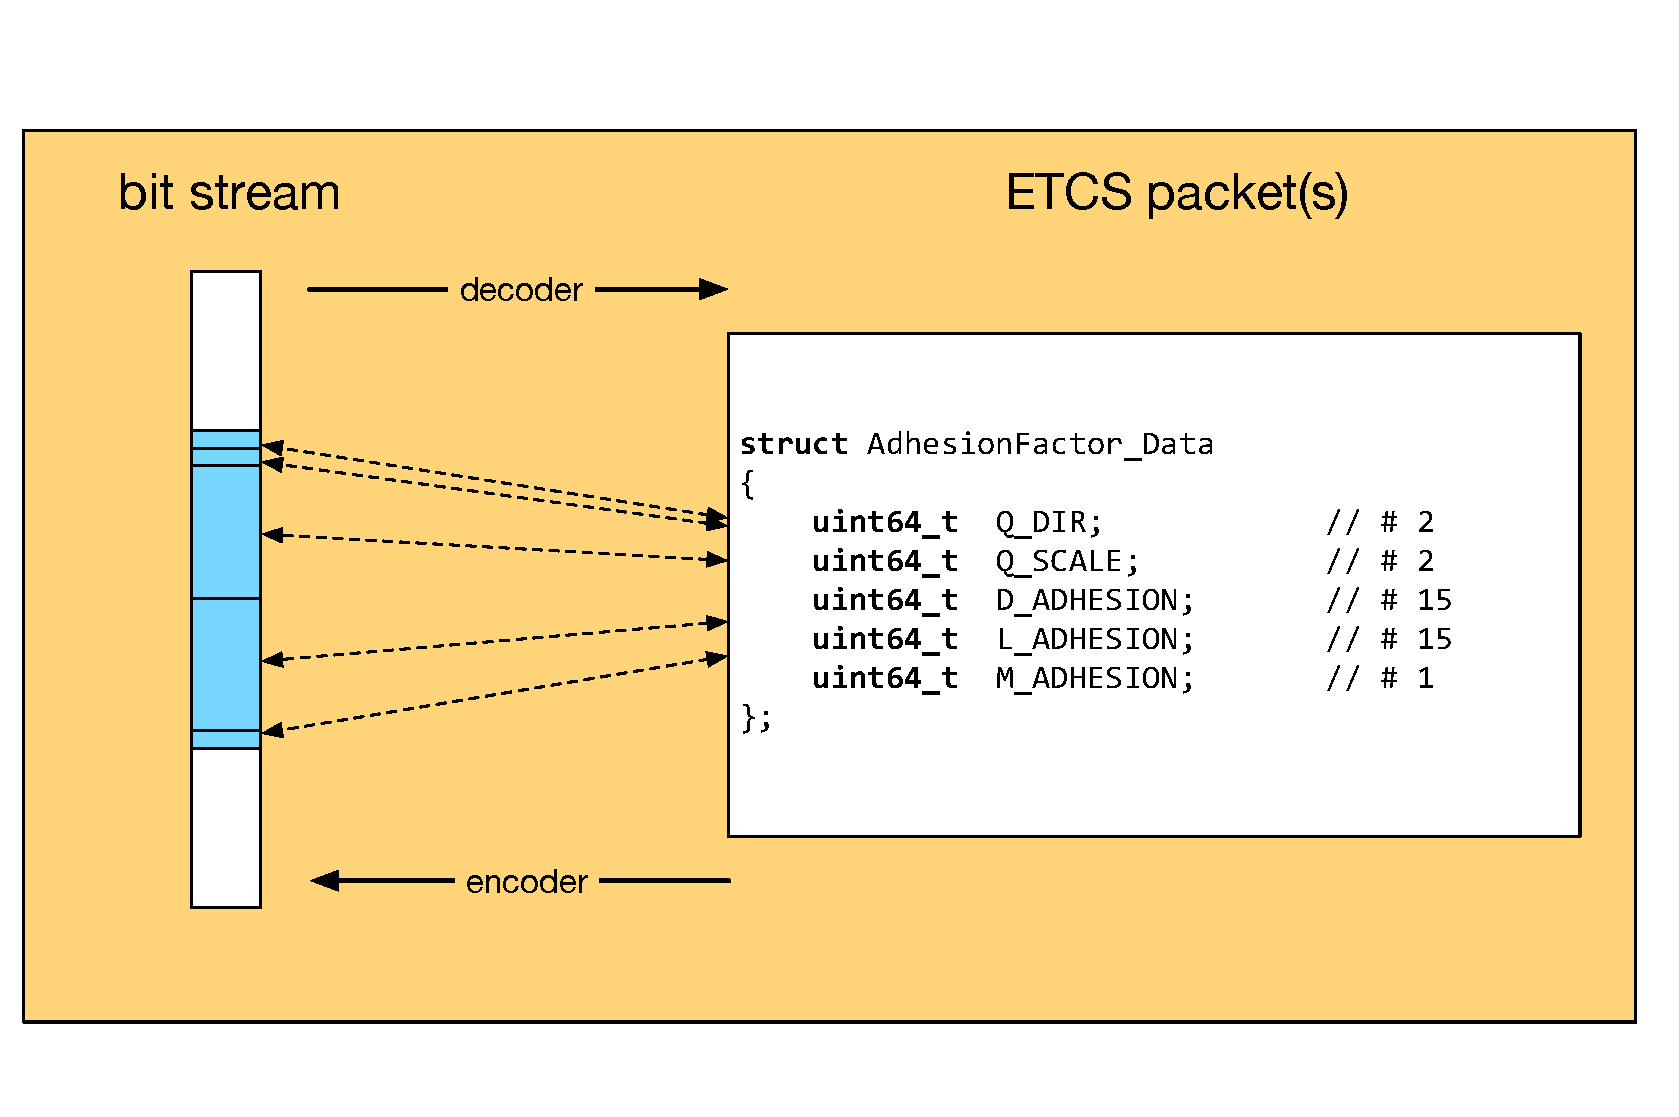
\includegraphics[width=0.99\textwidth]{figures/equalbits-adhesion.pdf}
\caption{\label{fig:adhesionfactor-bitstream}
        Relationship between bit stream and packet elements}
\end{center}
\end{figure}

\FloatBarrier  

\subsection{\acsl predicates \inl{AdhesionFactor}}
\label{sec:adhesionfactor-predicates-bitsize}

Listing~\ref{lst:adhesionfactor-predicates-bitsize} shows the definition of
the logic functions \inl{BitSize} and \inl{MaxBitSize} for \inl{AdhesionFactor}.
The former function uses a macro that contains the size of \inl{AdhesionFactor} in bits.
The functions are used in Listing~\ref{lst:adhesionfactor-decodebit} and
Listing~\ref{lst:adhesionfactor-encodebit} where the overloading of the
logic predicates allows for a more generic \acsl contract for the \inl{EncodeBit} and
\inl{DecodeBit} functions.

\begin{listing}[hbt]
\begin{minipage}{0.99\textwidth}
\begin{lstlisting}[style=acsl-block]
/*@
    logic integer BitSize{L}(AdhesionFactor* p) = ADHESIONFACTOR_BITSIZE;

    logic integer MaxBitSize{L}(AdhesionFactor* p) = BitSize(p);
*/
\end{lstlisting}
\end{minipage}
\caption{\label{lst:adhesionfactor-predicates-bitsize}Definition of the \inl{BitSize} predicates for \inl{AdhesionFactor}}
\end{listing}

\FloatBarrier

\label{sec:adhesionfactor-predicates-invariant}

Listing~\ref{lst:adhesionfactor-predicates-invariant} shows the definition of the
\inl{Invariant} predicate for \inl{AdhesionFactor}.
The predicate is the conjunction of the (trivial) \inl{Invariant(uint64_t)} predicates
of all members of on object of type \inl{AdhesionFactor}.

\begin{listing}[hbt]
\begin{minipage}{0.99\textwidth}
\begin{lstlisting}[style=acsl-block]
/*@
    predicate Invariant(AdhesionFactor* p) =
      Invariant(p->Q_DIR)             &&
      Invariant(p->L_PACKET)          &&
      Invariant(p->Q_SCALE)           &&
      Invariant(p->D_ADHESION)        &&
      Invariant(p->L_ADHESION)        &&
      Invariant(p->M_ADHESION);
*/
\end{lstlisting}
\end{minipage}
\caption{\label{lst:adhesionfactor-predicates-invariant}Definition of the \inl{Invariant} predicate for \inl{AdhesionFactor}}
\end{listing}

\FloatBarrier

\label{sec:adhesionfactor-predicates-upperbitsnotset}

%\fxfatal{Make sure that there is an explanation of UpperBitsNotSet in Chapter~\ref{cha:bitstream}}

Listing~\ref{lst:adhesionfactor-predicates-upperbitsnotset} shows the definition
of the \inl{UpperBitsNotSet} predicate for \inl{AdhesionFactor}.

\begin{listing}[hbt]
\begin{minipage}{0.99\textwidth}
\begin{lstlisting}[style=acsl-block]
/*@
    predicate UpperBitsNotSet(AdhesionFactor* p) =
      UpperBitsNotSet(p->Q_DIR,            2)   &&
      UpperBitsNotSet(p->L_PACKET,         13)  &&
      UpperBitsNotSet(p->Q_SCALE,          2)   &&
      UpperBitsNotSet(p->D_ADHESION,       15)  &&
      UpperBitsNotSet(p->L_ADHESION,       15)  &&
      UpperBitsNotSet(p->M_ADHESION,       1);
*/
\end{lstlisting}
\end{minipage}
\caption{\label{lst:adhesionfactor-predicates-upperbitsnotset}Definition of the \inl{UpperBitsNotSet} predicate for \inl{AdhesionFactor}}
\end{listing}

\FloatBarrier

The predicate \inl{UpperBitsNotSet(AdhesionFactor*)} holds
if and only if the values of all members of \inl{AdhesionFactor}
fit into their assigned numbers of bits.
The predicate is defined as the conjunction of the overloaded \inl{UpperBitsNotSet} predicate
which is explained in Section~\ref{sec:bit operations in framac}, for all members of \inl{AdhesionFactor}.

\label{sec:adhesionfactor-predicates-separated}

Listing~\ref{lst:adhesionfactor-predicates-separated} shows the definition of 
predicate  \inl{Separated} for \inl{AdhesionFactor}.
The predicate \inl{Separated(stream, p)} is true if and only if 
the two objects \inl{*stream} and \inl{*p} do not overlap in memory.
Thus, writing into the stream will not change \inl{*p} and vice versa.

\begin{listing}[hbt]
\begin{minipage}{0.99\textwidth}
\begin{lstlisting}[style=acsl-block]
/*@
    predicate Separated(Bitstream* stream, AdhesionFactor* p) =
      \separated(stream, p) &&
      \separated(stream->addr + (0..stream->size-1), p);
*/
\end{lstlisting}
\end{minipage}
\caption{\label{lst:adhesionfactor-predicates-separated}Definition of the \inl{Separated} predicate for \inl{AdhesionFactor}}
\end{listing}

\FloatBarrier

\label{sec:adhesionfactor-predicates-equalbits}

%\fxfatal{Make sure that there is an explanation of EqualBits in Chapter~\ref{cha:bitstream}}

Listing~\ref{lst:adhesionfactor-predicates-equalbits} shows the definition of the
\inl{EqualBits} predicate for \inl{AdhesionFactor}.
Based on the ETCS specification, this predicate describes a
relationship between the bits of the individual members
of an object of type \inl{AdhesionFactor} and those of a bit stream.
This predicate will be used to formally describe the transfer of bits
from a bit stream to an object of type \inl{AdhesionFactor} and vice versa.
The definition of the predicate \inl{EqualBits(AdhesionFactor*)} uses
the predicate \inl{EqualBits(uint64_t)}, which is explained
in Section~\ref{sec:bitstream}.

\begin{listing}[hbt]
\begin{minipage}{0.99\textwidth}
\begin{lstlisting}[style=acsl-block]
/*@
    predicate EqualBits(Bitstream* stream, integer pos, AdhesionFactor* p) =
      EqualBits(stream, pos,       pos + 2,   p->Q_DIR)             &&
      EqualBits(stream, pos + 2,   pos + 15,  p->L_PACKET)          &&
      EqualBits(stream, pos + 15,  pos + 17,  p->Q_SCALE)           &&
      EqualBits(stream, pos + 17,  pos + 32,  p->D_ADHESION)        &&
      EqualBits(stream, pos + 32,  pos + 47,  p->L_ADHESION)        &&
      EqualBits(stream, pos + 47,  pos + 48,  p->M_ADHESION);
*/
\end{lstlisting}
\end{minipage}
\caption{\label{lst:adhesionfactor-predicates-equalbits}Definition of the \inl{EqualBits} predicate for \inl{AdhesionFactor}}
\end{listing}

\FloatBarrier

\subsection{Formal specification of \inl{AdhesionFactor_UpperBitsNotSet}}
\label{sec:adhesionfactor-upperbitsnotset}

Listing~\ref{lst:adhesionfactor-upperbitsnotset} shows the contract of the \inl{UpperBitsNotSet}
function for \inl{AdhesionFactor}.

\begin{listing}[hbt]
\begin{minipage}{0.99\textwidth}
\begin{lstlisting}[style=acsl-block]
/*@
    requires valid:      \valid_read(p);
    requires invariant:  Invariant(p);

    assigns \nothing;

    ensures result:  \result <==> UpperBitsNotSet(p);
*/
int AdhesionFactor_UpperBitsNotSet(const AdhesionFactor* p);
\end{lstlisting}
\end{minipage}
\caption{\label{lst:adhesionfactor-upperbitsnotset}Contract for \inl{UpperBitsNotSet} function of \inl{AdhesionFactor}}
\end{listing}

\FloatBarrier

The function contract includes the \inl{requires} clauses, labeled \inl{valid} and \inl{invariant}.
These limit the significance of the \inl{ensures} and \inl{assigns} clauses to
the \inl{AdhesionFactor} objects that also satisfy the \inl{requires} clauses.
The \inl{valid} clause only evaluates to true if the \inl{*p} is a valid pointer.
The \inl{invariant} clause requires \inl{Invariant(p)} to evaluate to true.
The \inl{Invariant(AdhesionFactor*)} predicate is explained
in Section~\ref{sec:adhesionfactor-predicates-invariant}.
The contract also includes a statement on the return value of the function, labeled \inl{result}.
This clause ensures that the function's return value for \inl{AdhesionFactor* p}
matches the evaluation of the predicate \inl{UpperBitsNotSet(p)}
from Section~\ref{sec:adhesionfactor-predicates-upperbitsnotset}.
With the \inl{assigns \\nothing} clause the contract furthermore
specifies that this function has no side effects.

\clearpage

\subsection{Formal specification of \inl{AdhesionFactor_DecodeBit}}
\label{sec:adhesionfactor-decodebit}

Listing~\ref{lst:adhesionfactor-decodebit} shows the contract
for the \inl{DecodeBit} function for \inl{AdhesionFactor}.
The behavior of the function is specified using the
two disjoint behaviors \inl{normal_case} and \inl{error_case}.
The requirements \inl{valid_stream}, \inl{stream_invariant},
\inl{valid_package} and \inl{separation} apply to both behaviors
and limit the set of combinations of input arguments for which the
\inl{ensures} and \inl{assigns} clauses describe the behavior
of the function.

\begin{listing}[hbt]
\begin{minipage}{0.99\textwidth}
\begin{lstlisting}[style=acsl-block]
/*@
    requires valid_stream:      Readable(stream);
    requires stream_invariant:  Invariant(stream, MaxBitSize(p));
    requires valid_package:     \valid(p);
    requires separation:        Separated(stream, p);

    assigns stream->bitpos;
    assigns *p;

    ensures unchanged:          Unchanged{Here,Old}(stream, 0, 8*stream->size);

    behavior normal_case:
      assumes Normal{Pre}(stream, MaxBitSize(p));

      assigns stream->bitpos;
      assigns *p;

      ensures invariant:  Invariant(p);
      ensures result:     \result == 1;
      ensures increment:  stream->bitpos == \old(stream->bitpos) + BitSize(p);
      ensures equal:      EqualBits(stream, \old(stream->bitpos), p);
      ensures upper:      UpperBitsNotSet(p);

    behavior error_case:
      assumes !Normal{Pre}(stream, MaxBitSize(p));

      assigns \nothing;

      ensures result: \result == 0;

    complete behaviors;
    disjoint behaviors;
*/
int AdhesionFactor_DecodeBit(AdhesionFactor* p, Bitstream* stream);
\end{lstlisting}
\end{minipage}
\caption{\label{lst:adhesionfactor-decodebit}Contract for \inl{DecodeBit} function of \inl{AdhesionFactor}}
\end{listing}

\FloatBarrier


The \inl{assigns} clauses in the contract's body describe the
side effects of the function.
If the function contract is split into multiple behaviors,
like here, common \inl{assigns} clauses, which contain the union
of the behaviors' \inl{assigns} clauses, are needed outside
of the behaviors.
Their meaning will become clear when discussing the
individual  behaviors.

For both behaviors the \inl{unchanged} clause states that
none of the bits in the bit stream are written by the function.

\begin{itemize}
\item
The property \inl{valid_stream} requires that the predicate \inl{Readable(stream)}
is satisfied (see Section~\ref{sec:bitstream}).

\item
The property \inl{stream_invariant} is only met if the \inl{Invariant} predicate is true.
The predicate \inl{Invariant(Bitstream*, integer)} is described in
Section~\ref{sec:bitstream}.

\item
The property \inl{valid_package} requires that \inl{p} is a valid pointer for read and write operations.

\item
The property \inl{separation} requires that \inl{*stream} and \inl{*p} do not overlap in the memory.
The 
\inl{Separated}
predicate was introduced in
Section~\ref{sec:adhesionfactor-predicates-separated}.
\end{itemize}

The behavior \inl{normal_case} describes the function's behavior if
\inl{*stream} contains enough unread bits to fill
all members of \inl{*p}. 
In this case an object of type \inl{AdhesionFactor}
is decoded from the stream
and thus \inl{*p} is written.
The latter is stated by the first \inl{assigns} clause.
In this context the \inl{ensures} clauses \inl{equal} and \inl{upper}
describe the relationship of the bits in the bit stream and
the bits of the members of \inl{*p}.
Furthermore \inl{stream->bitpos} will be updated.
The effects of this operation are described by the second
\inl{assigns} and the \inl{increment} clauses.

The behavior \inl{error_case} describes the function's behavior in the opposite case
i.e. if \inl{*stream} is exhausted before all members of \inl{*p} are read.
In this case the function has no side effects and in particular does not write
\inl{*p} or \inl{stream->bitpos}.
The \inl{ensures} clause \inl{result} states that the return value
of the function equals \inl{0}. In \inl{normal_case} this value was specified to equal \inl{1}.

The distinguishing predicate for the two behaviors is \inl{Normal(Bitstream*, integer)},
which appears in the \inl{assumes} clauses within both behaviors and
is explained in Section~\ref{sec:bitstream}. 

\clearpage 

\subsection{Formal specification of \inl{AdhesionFactor_EncodeBit}}
\label{sec:adhesionfactor-encodebit}

Listing~\ref{lst:adhesionfactor-encodebit} shows the contract
for the \inl{EncodeBit} function for \inl{AdhesionFactor}.

\begin{listing}[hbt]
\begin{minipage}{0.99\textwidth}
\begin{lstlisting}[style=acsl-block]
/*@
    requires valid_stream:      Writable(stream);
    requires stream_invariant:  Invariant(stream, MaxBitSize(p));
    requires valid_package:     \valid_read(p);
    requires invariant:         Invariant(p);
    requires separation:        Separated(stream, p);

    assigns stream->bitpos;
    assigns stream->addr[0..(stream->size-1)];

    behavior normal_case:
      assumes Normal{Pre}(stream, MaxBitSize(p)) && UpperBitsNotSet{Pre}(p);

      assigns stream->bitpos;
      assigns stream->addr[0..(stream->size-1)];

      ensures result:     \result == 1;
      ensures increment:  stream->bitpos == \old(stream->bitpos) + BitSize(p);
      ensures left:       Unchanged{Here,Old}(stream, 0, \old(stream->bitpos));
      ensures middle:     EqualBits(stream, \old(stream->bitpos), p);
      ensures right:      Unchanged{Here,Old}(stream, stream->bitpos, 8 * stream->size);

    behavior values_too_big:
      assumes Normal{Pre}(stream, MaxBitSize(p)) && !UpperBitsNotSet{Pre}(p);

      assigns \nothing;

      ensures result:        \result == -2;

    behavior invalid_bit_sequence:
      assumes !Normal{Pre}(stream, MaxBitSize(p));

      assigns \nothing;

      ensures result:       \result == -1;

    complete behaviors;
    disjoint behaviors;
*/
int AdhesionFactor_EncodeBit(const AdhesionFactor* p, Bitstream* stream);
\end{lstlisting}
\end{minipage}
\caption{\label{lst:adhesionfactor-encodebit}Contract for \inl{EncodeBit} function of \inl{AdhesionFactor}}
\end{listing}

\FloatBarrier

The behavior of the function is described using the three
disjoint behaviors \inl{normal_case}, \inl{values_too_big}
and \inl{invalid_bit_sequence}.
The requirements \inl{valid_stream}, \inl{stream_invariant},
\inl{valid_package}, \inl{invariant} and \inl{separation}
are similar to those of the \inl{DecodeBit} function's
contract for \inl{AdhesionFactor}.
The ones not examined in detail here do not differ from
the ones in Section~\ref{sec:adhesionfactor-decodebit}.

Like for the \inl{DecodeBit} function for \inl{AdhesionFactor}
in Section~\ref{sec:adhesionfactor-decodebit} the \inl{assigns}
clauses in the contract body are the conjunction of the
\inl{assigns} clauses of the individual behaviors.

\begin{itemize}
\item
Property \inl{valid_stream} is only met if \inl{Writable(stream)} applies.
The predicate \inl{Writable(Bitstream*)} requires that the
stream is accessible for updates.
\item
Property \inl{valid_package} requires \inl{*p} to be valid pointer.
\item
Property \inl{invariant} is only met if the \inl{Invariant} predicate,
which was described in Section~\ref{sec:adhesionfactor-predicates-invariant},
holds for \inl{p}.
\end{itemize}

The behaviors of the \inl{EncodeBit} contract describe
one successful case and two error cases.

Behavior \inl{normal_case} describes a successful
encoding of the object \inl{*p} into the bit stream.
The \inl{assigns} clauses specify that in this case both
the \inl{bitpos} of the \inl{stream} and the fields
of the bit stream are written.
The \inl{increment} clause describes the new value for
\inl{bitpos}.
The \inl{ensures} clauses \inl{left}, \inl{middle}
and \inl{right} state that only some bits of the
bit stream are written.
The updated bits and their relationship to the
bits of the members of the object \inl{*p}
are described with the \inl{EqualBits} predicate,
which is described in
Section~\ref{sec:adhesionfactor-predicates-equalbits}.
The \inl{Unchanged} predicate specifies that the
bits in the bit stream before the old \inl{stream->bitpos}
and the after the new \inl{stream->bitpos}
remain unchanged.
\inl{Unchanged(Bitstream*, integer, integer)}
is defined in Section~\ref{sec:bitstream}.

Behavior \inl{values_too_big} describes
the scenario in which the value of at least one
member of \inl{*p} is bigger than the specified
bit size for that member of
\inl{AdhesionFactor} allows.
The numbers of bits for the members of
\inl{AdhesionFactor} are specified in
Section~\ref{sec:adhesionfactor-etcs}.
The \inl{assigns} clause states that this behavior
of the function causes no side effects and
the \inl{result} clause ensures that the
function will return the value \inl{-2}.
In contrast to \inl{normal_case},
for this behavior it is assumed that the
\inl{UpperBitsNotSet(p)} predicate evaluates
to false.
The \inl{Normal(stream, MaxBitSize(p))}
predicate returns true for both behaviors.

Finally, the behavior \inl{invalid_bit_sequence} describes the function's
behavior if the bit stream is not long enough to
write a complete \inl{AdhesionFactor} object
into. 
This behavior is distinguished from the other
behaviors by the evaluation of the predicate
\inl{Normal(stream, MaxBitSize(p))}.
Notice that the evaluation of \inl{UpperBitsNotSet(p)}
might be false, too.
Like in the \inl{value_too_big} behavior the function
ends without encoding any bits into the stream.
Therefore the \inl{assigns} clause is \inl{\\nothing}.
The \inl{result} clause states that the function's
return value equals \inl{-1}.

\clearpage

\section{Formal specification of other packets}
\label{sec:other-packets}

After examining the definition of the predicates for \inl{AdhesionFactor}
and the formal specifications of the functions \inl{AdhesionFactor_EncodeBit}
and \inl{AdhesionFactor_DecodeBit} from Section~\ref{sec:adhesionfactor},
the predicates for other (static) packets and the specifications of the corresponding
functions look very familiar.

In fact the only difference of the predicates lies in the different
sets of sub predicates which are used and depends on the different sets
of member variables for the different packets.
The fact that \acsl predicates and logic functions can be \emph{overloaded}
for different types enables us to develop \emph{generic}
formal specifications for the
\inl{EncodeBit} and \inl{DecodeBit} functions of all packets.

